\ifSTANDALONE
\section{Brushless Motoransteuerung}
\fi
\ifEMBED
\subsubsection{Brushless Motoransteuerung}
\fi

\ifEMBED
    % Dieses Kapitel ist eine Zusammenarbeit der Gruppen \BLDCTeams. 
    \BLDCcollab
\fi
\ifSTANDALONE
    \subsection{Theorie der Ansteuerung}
    \fi
\ifEMBED
    \paragraph{Theorie der Ansteuerung}$~~$\\
    \fi
    \ifEMBED
        \begin{wrapfigure}{r}{0.50\textwidth}
           	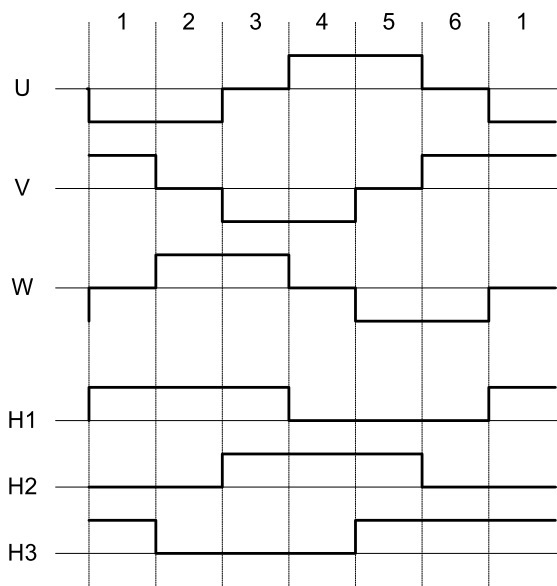
\includegraphics[scale=0.50,clip,trim=2mm 0mm 0mm 0mm]
           	{\EtPath/Bilder/ZeitlicheHallSensorAnsteuerung.jpg}
         	\centering
           	\caption[Zeitliche Darstellung der Ansteuerung mit Hall-Sensoren]
           	{Zeitliche Darstellung der Ansteuerung mit Hall-Sensoren \cite{AppNote:BrushlessuC}}
            \label{abb:ZeitlicheAnsteuerungBrushlessMotor}
        \end{wrapfigure}
    \fi
        Brushless-Motoren (BLDC-Motoren) sind Synchron-Drehstrom-Motoren. Das 
        bedeutet, sie werden mittels eines kontinuierlichen magnetischen 
        Drehfeldes in Bewegung gesetzt.  Dabei ist darauf zu achten, dass der 
        Läufer dem Drehfeld synchron folgen kann, daher auch die 
        Namensbezeichnung des Motors. Falls der Läufer dem Drehfeld nicht 
        folgen kann, wird keine Spannung vom Rotor in die Statorwicklung 
        induziert, die der Erregerspannung entgegenwirkt. Daraus folgt, dass 
        ein immenser Strom fliesst, der nur von der Wicklungsimpedanz des 
        Motors begrenzt wird. Das Drehmoment ist abhängig vom Polradwinkel und 
        erreicht sein Maximum bei einem Polradwinkel von 90$^\circ$. Die 
        Kommutierung wird entweder als Sinuskommutierung oder als 
        Blockkommutierung ausgeführt. Die Sinuskommutierung bildet die 
        Sinusform eines dreiphasigen Netzes nach. Die Sinusform kann mit einem 
        Rechtecksignal angenähert werden. Dabei spricht man von einer 
        Blockkommutierung. Diese ist einfacher zu realisieren, aber erreicht 
        nicht das selbe Drehmoment wie eine Sinuskommutierung. In diesem 
        Projekt wird aufgrund der einfacheren Implementierung eine 
        Blockkommutierung realisiert. \\
    \ifSTANDALONE
        \begin{figure}[h!]
            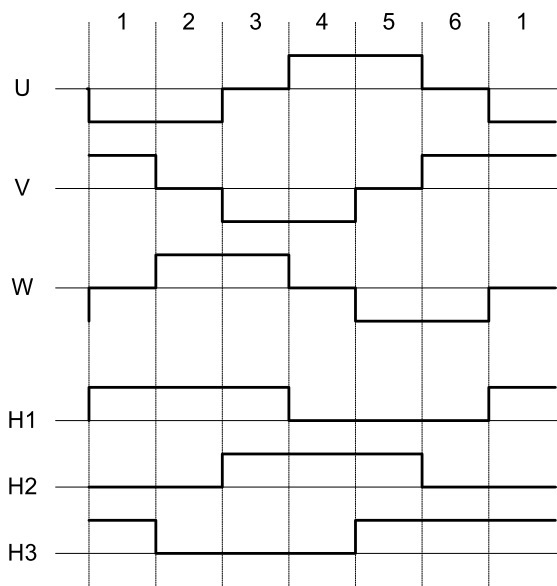
\includegraphics[scale=0.45]{\EtPath/Bilder/ZeitlicheHallSensorAnsteuerung.jpg}
            \centering
            \caption[Zeitliche Darstellung der Ansteuerung mit Hall-Sensoren]
            {Zeitliche Darstellung der Ansteuerung mit Hall-Sensoren \cite{AppNote:BrushlessuC}}
            \label{abb:ZeitlicheAnsteuerungBrushlessMotor}
        \end{figure}
    \fi
        \\
        Es gibt hauptsächlich drei Methoden das Drehfeld zu generieren und zu 
        regeln. Die einfachste Methode ist die Zwangskommutierung: 
        Dabei wird ein Drehfeld erzeugt und dem Motor aufgezwungen. Der Läufer 
        muss dem Drehfeld folgen, der maximal zulässige Winkel von 90$^\circ$
        zwischen dem Feld und dem Läufer muss eingehalten werden. Wird dieser 
        Winkel überschritten, kommt der Motor zum Stillstand.\\
        \\
        Die zweite Methode zur Regelung des Motors verwendet drei Hallsensoren, die im 
        Motor integriert sind. Dies macht den Motor aufwändiger und 
        dementsprechend teurer. Die Regelung mit Hallsensoren ist 
        verhältnismässig einfach, da nach den Signalen die einzelnen Spulen 
        direkt angesteuert werden können. Der Zusammenhang zwischen der 
        Ansteuerung und den Hallsensor-Signalen ist in Abbildung 
        \ref{abb:ZeitlicheAnsteuerungBrushlessMotor} ersichtlich. Dabei stehen 
        $U$, $V$ und $W$ für die Phasenströme und $H_1$, $H_2$ und $H_3$ für die 
        entsprechenden Signale der Hallsensoren. Aus dieser Darstellung ist 
        ersichtlich, dass wenn ein Hallsensor eine Änderung anzeigt, 
        ein Nulldurchgang im entsprechenden Stromverlauf stattgefunden hat. 
        Dies ist der Zeitpunkt, zu dem die Kommutierung durchgeführt werden 
        muss.\\
        \\
        Für die dritte Möglichkeit bildet man einen virtuellen Sternpunkt 
        und detektiert mit Komparatoren die Sternpunktdurchgänge. 
        In der Controller-Logik muss der Zeitunterschied der Kommutierung 
        bis zum Durchschreiten des Sternpunktes gemessen werden. Diese Zeit 
        muss noch einmal abgewartet werden, bevor die Kommutierung durchgeführt 
        wird. Falls der Motor über einen Anschluss für den Sternpunkt 
        verfügt, kann auch dieser verwendet werden. Da die Position des Rotors 
        auf diese Weise beim Stillstand nicht ermittelt werden kann, muss der 
        Motor mit einer Zwangskommutierung gestartet werden. 
\ifSTANDALONE
    \subsection{Neuer Ansatz}
\fi
\ifEMBED
    \paragraph{Neuer Ansatz}$~~$\vspace{2mm}\\
    \fi
%    \ifEMBED
%        \begin{wrapfigure}{r}{0.4\textwidth}
%            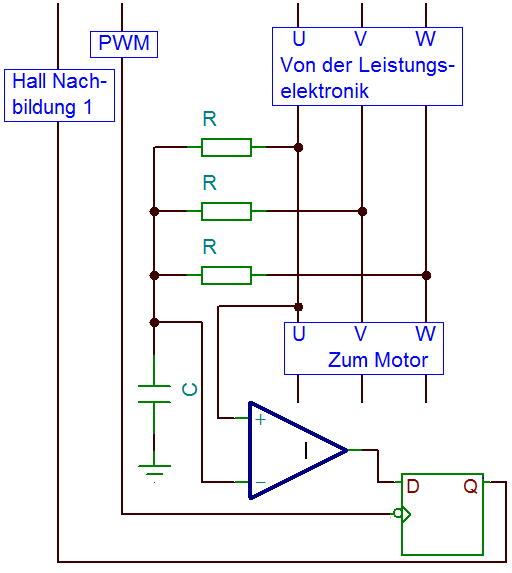
\includegraphics[scale=0.5]{\EtPath/Bilder/PrinzipDerRekonstruktion.png}
%            \centering
%            \caption[Schema des Rekonstruktionsprinzip]{Schema des Rekonstruktionsprinzip \cite{HSLU:Pluess}}
%            \label{abb:PrinzipRekonstruktion}
%%            \vspace{1cm}
%        \end{wrapfigure}
%    \fi
        In einem modifizierten Ansatz wird versucht, die Hallsensor-Signale 
        aus den Ansteuerungen des Motors zu gewinnen. Hierzu wird 
        eine Schaltung pro Phase benötigt, um die Nulldurchgänge beim 
        virtuellen Sternpunkt detektieren zu können. Die Abbildung 
        \ref{abb:PrinzipRekonstruktion} zeigt die Schaltung, mit der dieser Ansatz 
        realisiert werden kann. 
%    \ifSTANDALONE
    	\begin{figure}[h!]
            \centering
            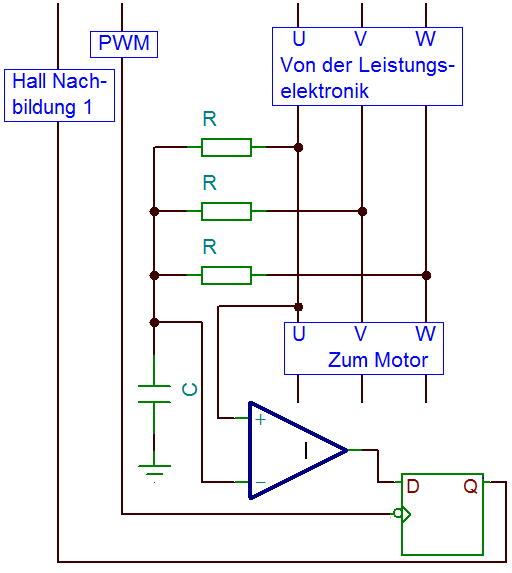
\includegraphics[scale=0.46]{\EtPath/Bilder/PrinzipDerRekonstruktion.png}
           	\caption{Schema des Rekonstruktionsprinzip \protect\cite{HSLU:Pluess}}
            \label{abb:PrinzipRekonstruktion}
        \end{figure}
%    \fi
        Mit dem Flip-Flop aus Abbildung \ref{abb:PrinzipRekonstruktion} kann die PWM aus dem 
        Sensorsignal unterdrückt werden. Diese rekonstruierten 
        Hallsensor-Signale können direkt logisch verknüpft und genutzt 
        werden, um den Motor mit einer Dreiphasen-H-Brücke anzusteuern 
        \cite{HSLU:Pluess}. Anhand des zeitlichen Verlaufs, der aus Abbildung 
        \ref{abb:ZeitlicheAnsteuerungBrushlessMotor} zu entnehmen ist und der 
        Ansteuerung einer H-Brücke, ergibt sich die Wahrheitstabelle, die in 
        Tabelle \ref{abb:WahrheitstabelleAnsteuerung} ersichtlich ist. Das 
        Signal $U_h$ symbolisiert den Highside\footnote{Transistor, der gegen 
        die Versorgungsspannung schaltet. Typischerweise aufwendiger 
        anzusteuern, da am Gate eine Spannung von einigen Volt über der 
        Versorgungsspannung angelegt werden muss. }-Transistor der Phase U auf der 
        H-Brücke und die Spalte $U_l$ entspricht dem Lowside-Transistor.\\      
        
        \begin{table}[h!]
            \begin{tabular}{ccc||cc|cc|cc||c}
                 $H_1$ & $H_2$ & $H_3$ & $U_h$ & $U_l$ & $V_h$ & $V_l$ & $W_h$ & $W_l$ & Illegal\\
            \hline 0   &   0   &   0   &   0   &   0   &   0   &   0   &   0   &   0   &   1\\
                   0   &   0   &   1   &   0   &   0   &   0   &   1   &   1   &   0   &   0\\
                   0   &   1   &   0   &   0   &   1   &   1   &   0   &   0   &   0   &   0\\
                   0   &   1   &   1   &   0   &   1   &   0   &   0   &   1   &   0   &   0\\
                   1   &   0   &   0   &   1   &   0   &   0   &   0   &   0   &   1   &   0\\
                   1   &   0   &   1   &   1   &   0   &   0   &   1   &   0   &   0   &   0\\
                   1   &   1   &   0   &   0   &   0   &   1   &   0   &   0   &   1   &   0\\
                   1   &   1   &   1   &   0   &   0   &   0   &   0   &   0   &   0   &   1\\
            \end{tabular}
           	\centering
           	\caption{Wahrheitstabelle der Ansteuerung} 
            \label{abb:WahrheitstabelleAnsteuerung}
        \end{table}
        \newpage
        \parindent 0pt Die Tabelle in Abbildung 
        \ref{abb:WahrheitstabelleAnsteuerung} kann pro Signal zu folgenden 
        logischen Verknüpfung vereinfacht werden\\
        \\
    \ifSTANDALONE
        \begin{table}
            \centering
            \begin{tabular}{ccc}
                $U_h = H_1 \wedge \bar{H_2}$ & $V_h = H_2 \wedge \bar{H_3}$ & $W_h = \bar{H_1} \wedge H_3$\\
                $U_l = \bar{H_1} \wedge H_2$ & $V_l = \bar{H_2} \wedge H_3$ & $W_l = H_1 \wedge \bar{H_3}$
            \end{tabular}
        \end{table}
    \fi
    \ifEMBED
        \begin{tabular}{ccc}
            $U_h = H_1 \wedge \bar{H_2}$ & $V_h = H_2 \wedge \bar{H_3}$ & $W_h = \bar{H_1} \wedge H_3$\\
            $U_l = \bar{H_1} \wedge H_2$ & $V_l = \bar{H_2} \wedge H_3$ & $W_l = H_1 \wedge \bar{H_3}$
        \end{tabular}
    \fi
    \ifSTANDALONE
    \subsection{Ansteuerungshardware}
    \fi
    \ifEMBED
    \paragraph{Ansteuerungshardware}$~~$\vspace{2mm}\\
    \fi
        In Kapitel \ref{chap:VersuchsResultat} zeigten sich einige Punkte, die für ein eigenes Board 
        für die Brushless-Motoransteuerung sprechen. Auf diesem Board wird ein eigener Controller 
        eingesetzt, der als Kommunikationsschnittstelle SPI verwendet. Die benötigten Pins sind in 
        der Tabelle \ref{abb:SchnittstelleBrushlessBoard} ersichtlich. Der Controller wird benötigt, 
        um eine Zwangskommutierung vorzunehmen, um den Motor in eine Initialdrehung zu versetzen. 
        Sobald der Motor dreht, kann der neue Ansatz funktionieren. Weiter wird auf dem Controller eine 
        Regelung implementiert, um die Drehzahl des Motors zu regeln. Zusätzlich kann der Winkel 
        zwischen Detektion und Kommutierung angepasst werden, wenn dies notwendig ist.\\
        \\
        Die Kommunikation mit dem Controller soll über SPI erfolgen. Darüber sollen die Solldrehzahl 
        und gegebenenfalls Parameter eingestellt werden können. Alle weiteren Schritte, wie die benötigte 
        Zwangskommutierung am Anfang und die Regelung, werden eigenständig vom Boardcontroller vorgenommen.
        %
        \begin{table}[h!]
            \begin{tabular}{ll}
                Pin     & Funktion \\
            \hline  SCK & Bustakt \\
                MISO    & Master in Slave out \\
                MOSI    & Master out Slave in \\
                CS      & Chip select \\
                Int     & Interrupt \\
                Reset   & Reset \\
            \end{tabular}
           	\centering
           	\caption{Schnittstelle des Brushless-Boards} 
            \label{abb:SchnittstelleBrushlessBoard}
        \end{table}
